% Embedded Systems Project Report

% Preamble: contains document parameters, like font size, document class, paper size, page layout, etc.
% Some of the packaged needed by the template provided must be installed using MikTex package manager

\documentclass[12pt, english]{scrartcl}
\usepackage[a4paper,bindingoffset=0.2in,left=.5in,right=.5in,top=1in,bottom=1in,footskip=.5in]{geometry}
\usepackage[english]{babel}
\usepackage{graphicx}
\usepackage{lipsum}
\usepackage[bitstream-charter]{mathdesign}
\usepackage[T1]{fontenc}
\graphicspath{{./figures/raster/}{./figures/vector/}}

\usepackage{tabularx}
\usepackage{array}
\newcolumntype{L}[1]{>{\raggedright\let\newline\\\arraybackslash\hspace{0pt}}m{#1}}
\newcolumntype{C}[1]{>{\centering\let\newline\\\arraybackslash\hspace{0pt}}m{#1}}
\newcolumntype{R}[1]{>{\raggedleft\let\newline\\\arraybackslash\hspace{0pt}}m{#1}}
\newcolumntype{P}[1]{>{\raggedleft\arraybackslash}p{#1}}

\usepackage{textcomp}
\usepackage{xcolor}
\usepackage{mathtools}
\usepackage{numprint}
\usepackage{amsmath}
\usepackage[linesnumbered]{algorithm2e}
\usepackage{multirow}
\usepackage{multicol}
\usepackage{subcaption}
\usepackage{float}

\usepackage{prettyref}
\newrefformat{fig}{Figure~\ref{#1}}
\newrefformat{tab}{Table~\ref{#1}}
\newrefformat{sec}{Section~\ref{#1}}
\newrefformat{ssec}{Paragraph~\ref{#1}}
\newrefformat{eq}{Equation~\ref{#1}}
\newrefformat{alg}{Algorithm~\ref{#1}}

\makeatletter
\newcommand{\redub}{}
\def\redub#1{%
  \@ifnextchar_%
    {\@redub{#1}}
    {\@latex@warning{Missing argument for \string\redub}\@redub{#1}_{}}%
}
\def\@redub#1_#2{%
    \colorlet{currentcolor}{.}%
    \color{black}%
    \underbrace{\color{currentcolor}#1}_{\color{black}#2}%
    \color{currentcolor}%
}
\makeatother

%----------------------------------------------------------------------------------------
%	My Info
%----------------------------------------------------------------------------------------
\newcommand{\horrule}[1]{\rule{\linewidth}{#1}}
\title{\normalfont \normalsize 
\textsc{Politecnico di Milano - Department of Electronics, Information and Bioengineering} \\[1cm]

\includegraphics[scale=1.2]{polimi} \\[1cm]
\horrule{0.5pt} \\[0.4cm]
\huge \textbf Porting of Miosix OS into a Vehicle Electronic Speed Control Board for Permanent Magnet Alternating Current Motors \\[.5cm] % The assignment title
\large Coding Project \\ % Pick one: Monography and Coding Project
\horrule{2pt} \\[0.5cm]
\vfill
\author{}
\begin{tabular}{r l}
\textbf{Student} & Arturo Montufar Arreola \\
\textbf{ID} & 840541 \\[0.5cm]
\textbf{Course} & Embedded Systems \\
\textbf{Academic Year} & 2016-2017 \\[0.5cm]
\textbf{Advisor} & Federico Terraneo \\ %e.g. Simone Libutti, Giuseppe Massari
\textbf{Professor} & William Fornaciari \\
\end{tabular}
\date{\normalsize\today}
}



\begin{document} % Anything between \begin{} and \end{} is called "environment"

	\maketitle % Print the title

	\pagebreak\tableofcontents\pagebreak

	\section{Introduction}
%\textbf{Hello, I'm a citation! \cite{mathes1976designing}.}
This project consisted in the porting of the Miosix Operating System for embedded devices into a vehicle electronic speed control (VESC) board, based on a STM32F405 microcontroller and designed to control permanent magnet alternating current motors. The main intention of the project was to prove the versatility of Miosix, creating and setting up a new board in the Kernel with a different hardware configuration, modifying the source code the least possible and creating new modules to successfully implement a Six-Step control of a brushless DC motor, which is one of the most efficient and accurate motor technologies available for applications which require high speed and high torque, but also its control is more complex than the control for other types of motors.


\subsection{Problem statement}
%\textbf{Hello, I'm another citation! \cite{miller1979humanistic}}.
Nowadays, electric motors are required in a large number and variety of industrial and domestic applications, from blenders and photographic cameras, to cars and power generation engines. As the complexity of the application increases, also the need for accuracy and efficiency does, leading to the development of different electric motor technologies and, therefore, different motion control techniques.\\

%TODO: Add reference to a book with Maxwell equations
To understand the problem being faced, it's necessary to briefly explain the basics of the electric motor. An electric motor is a device that transforms electric energy into mechanical energy by circulating a current in a rigid loop (i.e. an energized copper wire winding) under a magnetic field. The principle behind this is mainly explained by the Lorentz equation for the magnetic force

\begin{equation}
\overrightarrow{F_{B}}=q\overrightarrow{v}\times\overrightarrow{B}
\end{equation}

which states that the magnetic force $\overrightarrow{F_{B}}$ applied over a charged particle is equal to the charge of the particle $q$ multiplied by its velocity $\overrightarrow{v}$ and the magnetic field $\overrightarrow{B}$ acting over it in a perpendicular direction respect to its velocity. The rigid loop used to explain this principle is a rectangular shaped loop, able to spin in one of the axes of the plane where it's placed. In figure 1 we can see that a current $I$ flows though the loop in two situations: in figure 1.a, a magnetic field is orthogonal to the vector $\overrightarrow{S}$, which is normal to the plane of the loop; in figure 1.b, the magnetic field is parallel to the vector $\overrightarrow{S}$. \\

\begin{figure}[H]
 
\begin{subfigure}{.5\textwidth}
\centering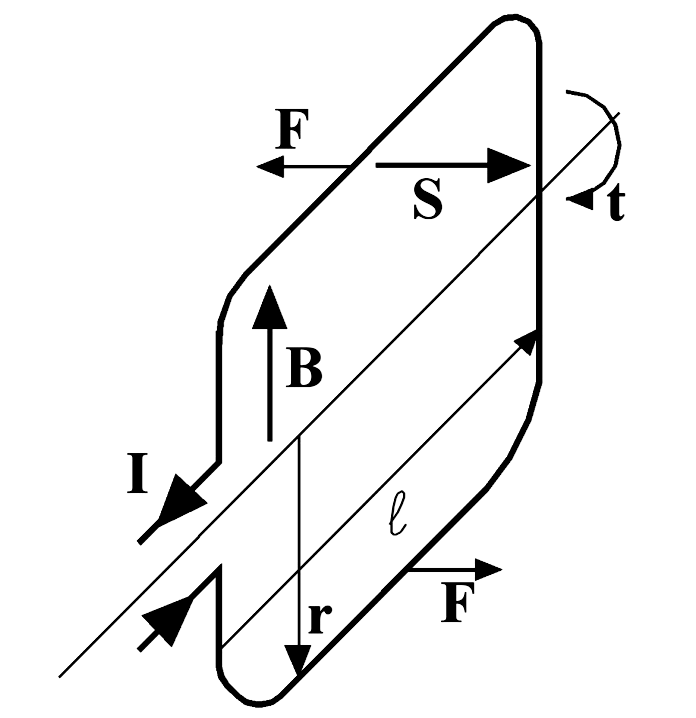
\includegraphics[width=.4\linewidth]{LorentzDiagram_a} 
\caption{$\overrightarrow{S}$ perpendicular to $\overrightarrow{B}$}
\label{fig:LorentzDiagram_a}
\end{subfigure}
\begin{subfigure}{.5\textwidth}
\centering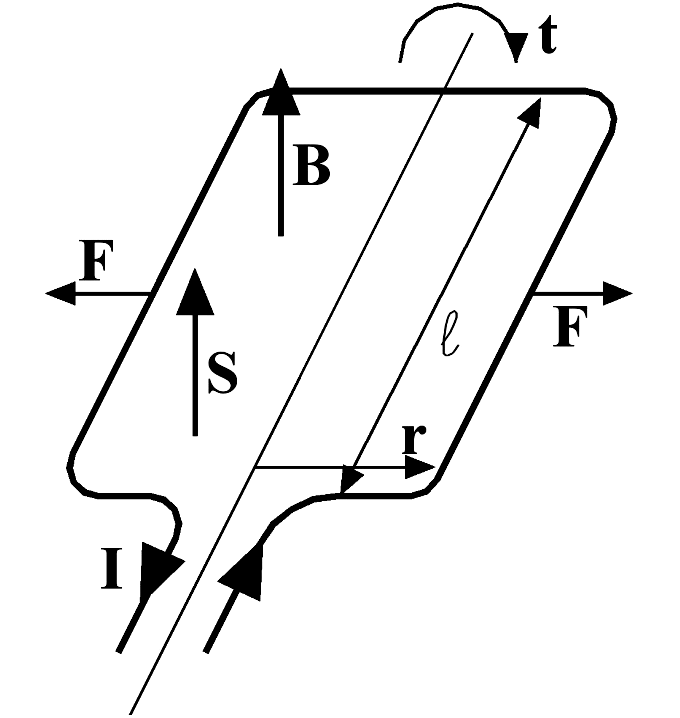
\includegraphics[width=.4\linewidth]{LorentzDiagram_b}
\caption{$\overrightarrow{S}$ parallel to $\overrightarrow{B}$}
\label{fig:LorentzDiagram_b}
\end{subfigure}
 
\caption{Torque on a conducting wire loop inside a magnetic field.}
\label{fig:Lorentz_diagrams}
\end{figure}

Following equation 1, we can see that there is a force applied to the sides of the loop where the circulating current is perpendicular to the magnetic field, therefore, there is torque applied in the axis where the loop can spin. In figure 1.a we can easily recognize the torque by considering 2 forces pushing the opposite sides of the loop into opposite directions. The opposite directions of the forces applied are defined by the direction of the circulating current. After reaching the maximum angle by pushing these sides of the loop, we reach the position shown on figure 1.b where there is no torque due to the overlap of the generated force vectors.\\

To overcome this situation where the coil doesn't move because there is no torque, and to create a continuous motion with a continuous torque, different solutions are provided, like the DC motor which uses multiple current loops and changes the direction of the current in each loop by using brushes and mechanical commutators, or the stepper motors and the permanent magnet AC motors, which instead of moving the energized coil under a static magnetic field, rotate a static magnetic field attached to the rotor by changing the current direction in the three-phase winded stator coils generating a rotating magnetic field which interacts with the static magnetic field "attached" to the rotor.

\begin{figure} [H]
\centering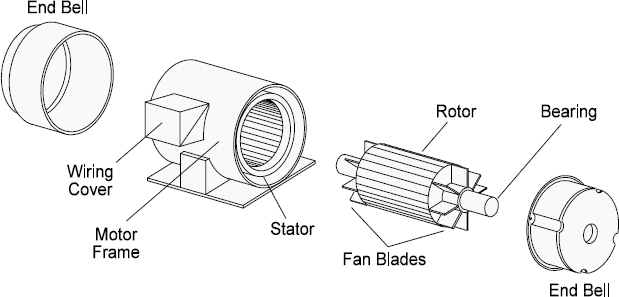
\includegraphics[width=10cm]{bldcAssembly}
\caption{Assembly details of a typical AC induction motor.}
\label{fig:PMAC_assembly}
\end{figure}

The motor used in this project was a Brushless DC (BLDC) motor, which is part of the family of the Permanent Magnet Alternating Current (PMAC) motors. The PMAC motors are preferred in some high speed applications over the DC motors because they have a longer life, they don't require maintenance and they don't generate sparks, which might be dangerous in some environments. These motors consist mainly on 3 components as shown in figure 2: the rotor, which has permanent magnets attached to it; the stator, which has the current carrying coils winded to it; and the end bells, which attach the rotor and the stator using bearings. As mentioned before, the motion of the motor is generated by the interaction between the static magnetic field of the permanent magnets in the rotor and a rotating magnetic field in the stator controlled by the current flowing through the coils winded in it. The different configurations of the coils winding in the stator define two types of motors: the BLDC motor, which has trapezoidal back-electromotive force (BEMF, which is the voltage generated in the coils due to the rotation of the magnetic field inside the windings loop, which creates a current that opposes to the movement of the magnetic field, as stated by Lenz Law) and the permanent magnet synchronous motor (PMSM), which has sinusoidal BEMF. Since the motor coil driving current should be shaped according to the shape of its BEMF, the BLDC motor is widely used because its driving signal is easier to implement due to the trapezoidal shape of its BEMF which can be generated by just alternating polarities in a three-phase inverter, while the PMSM needs a more complex algorithm to generate a three-phase sinusoidal signal. In some applications it's preferred to use PMSM because they can reach efficiencies up to 97\% and their drive generates lower harmonic components than the BLDC drive.\\ 

\begin{figure} [H]
\centering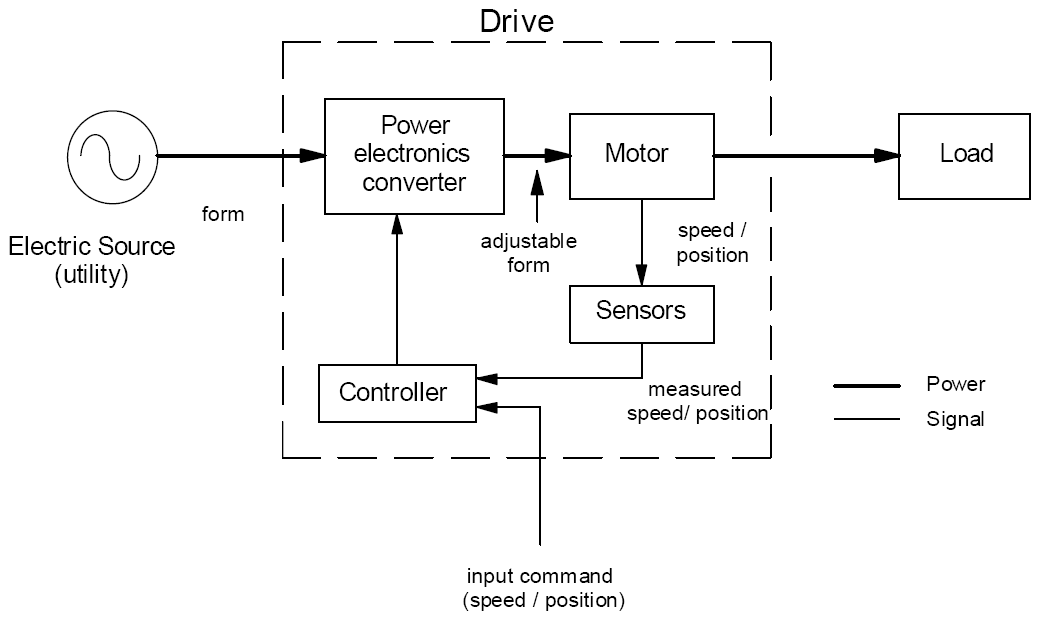
\includegraphics[width=12cm]{ElectricDrive}
\caption{Main components of an electric drive.}
\label{fig:Electric_Drive}
\end{figure}

%\textbf{Hello, I'm another citation! \cite{miller1979humanistic}}. 
%TODO: add reference to a work by Ghioni
The systems employed to control the motion of electric motors are called electric drives. The electric drive can be defined as an electromechanical device that deals with the conversion of electrical energy into mechanical energy to impart motion to different machines and mechanisms for various kinds of process control. In the case of the BLDC motors, the electric drive consists mainly in a three-phase inverter that generates a square signal depending on the wanted speed of rotation and the angular position of the rotor. Since the movement of its rotor depends on the position of its magnetic field, we need to detect its angular position to correctly drive the coils, therefore, depending on the position of the rotor, a sequence must be followed to rotate it. There are different methods to detect the rotor angular position, but the simplest one for the BLDC motor is to use Hall-effect sensors, which are normally attached to the stator and detect the magnetic field of the rotor. \\

\begin{figure} [H]
\centering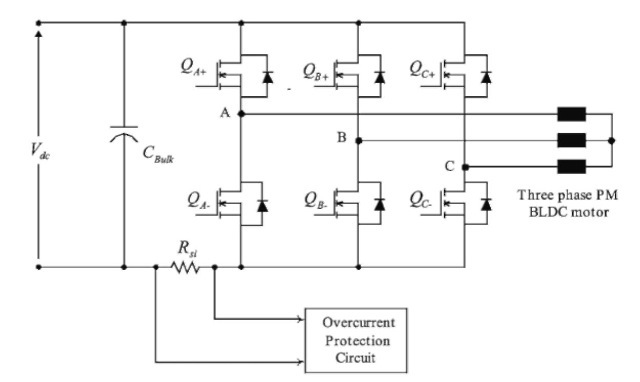
\includegraphics[width=12cm]{bldcInverter}
\caption{Three phase inverter consisting in 3 half-bridge inverters.}
\label{fig:BLDC_Inverter}
\end{figure}

The simplest driving method for this type of motors is called Six-Step drive, and consists in energizing each winding of the three-phase system for 120 degrees and leaving the winding de-energized for 60 degrees. To achieve this, a three-phase inverter is used. This three-phase inverter consists in 3 half-bridges which are driven following a six-steps commutation sequence that develops the most amount of torque possible according to the rotor position detected by the previously mentioned Hall-effect sensors. The motor is driven by energizing 2 phases at a time (current enters the first winding and exits the second winding) and leaving the third phase floating. In order to keep the motor running, the magnetic field produced by the windings should shift position, as the rotor moves to catch up with the stator field.

\begin{figure} [H]
\centering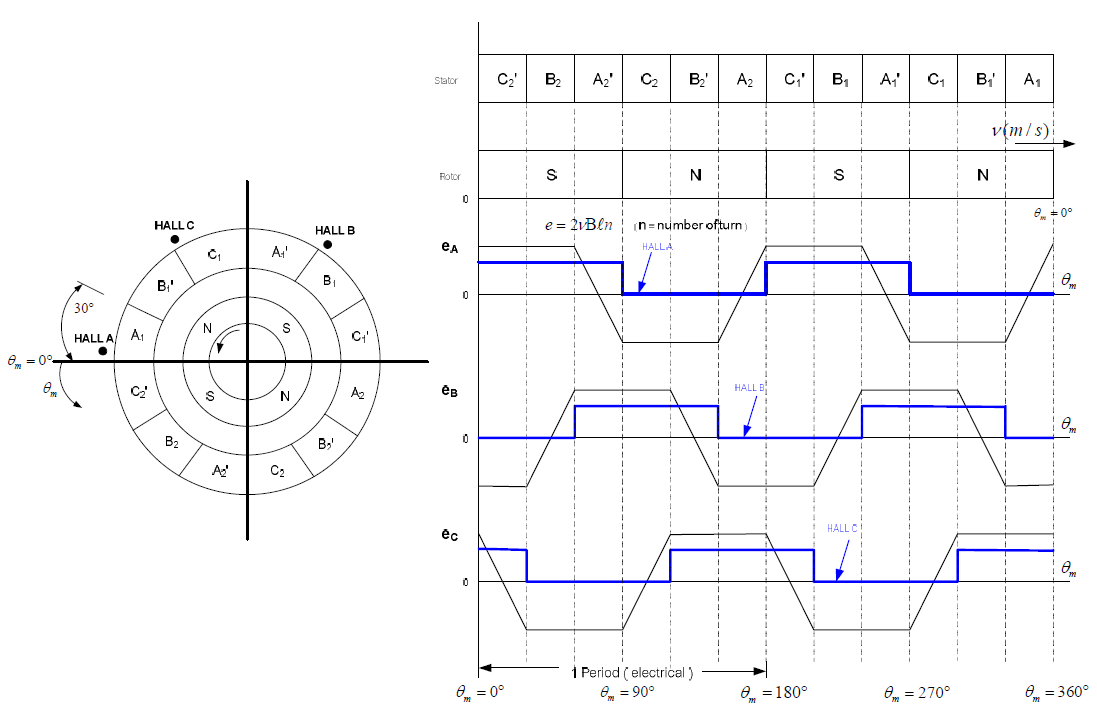
\includegraphics[width=16cm]{DriveDiagram}
\caption{At every 60 electrical degrees of rotation of the rotor's magnetic field, there is a change in the state of the hall sensors.}
\label{fig:BLDC_pulses_sequence}
\end{figure}

Since the driving methods for the PMSM are not trivial at all, specialized embedded systems must be developed to deal with the data acquisition and motor driving in an effective, versatile, robust and fast way. The embedded systems that deal with this kind of motors are normally called Electronic Speed Controllers (ESC), and its main purpose is to vary the electric motor's speed and direction. These ESC circuits consist mainly in the following components: a processing unit, normally a microcontroller, which will control the system according to the reference value wanted and the conditions of the motor which are sensed by the same; the driver circuit, which consists in an interface between the microcontroller and the power transistors that energize the coils; the power transistors, which are selected according to the power requirements of the application; and the data acquisition module, which consists mainly in rotor angular position detection or the Hall-effect signal conditioning and the current sensors that are used to avoid overcurrent problems. \\

To deal with all the information mentioned previously, the microcontroller for the application must be selected carefully, considering the speed of the motor, the accuracy and efficiency needed for the system and the external functionalities needed depending on the application. Together with the selection of the device, the software of the embedded system must be developed to manage to obtain the desired performance, which leads to the development of more complex algorithms and operating systems to run inside the embedded system.

\subsection{Summary of the work}
To 
\lipsum[2]

\pagebreak

\section{Design and implementation}
\textbf{Please make sure you explicitely cite the figures.
\prettyref{fig:polimi_logo} shows the logo of Politecnico di Milano.
Please also make sure you provide each figure with an exhaustive caption.}

\lipsum[1-12]



\section{Experimental evaluation}
\lipsum[1]
\subsection{Experimental setup}
\lipsum[1-2]
\subsection{Results}
\textbf{Please make sure you explicitely cite the tables.
\prettyref{tab:a_complex_table} shows a complex table.
Please also make sure you provide each table with an exhaustive caption.
Captions for tables must be placed before not after the tables.}
\lipsum[1-4]


\begin{table}
\small
\begin{center}

\caption{Summary of the test scenarios.
$M_1\xrightarrow{\alpha}M_2$ means that an application mapping
is changed from $M_1$ to $M_2$ after application $\alpha$
has terminated.}
\begin{tabular}{l|lcc|L{2cm}l}
\cline{2-6}
& \multicolumn{3}{c|}{Description of the workload} & \multicolumn{2}{c}{Cores allocation}\\
\cline{2-6}
Name of scenario & Application & Threads & $\frac{Threads}{Cores}$ & HMP & HMP w/policy \\
\hline

\multirow{2}{*}{LITTLE 1} & ferret$\dagger$ & 1 & \multirow{2}{*}{1.00} & $0-3$ & $0$ \\
 & vips & 3 & & $0-3$ & $1-3 \xrightarrow{\dagger} 0-3$ \\
\hline
\multirow{2}{*}{LITTLE 2} & freqmine$\dagger$ & 2 & \multirow{2}{*}{1.25} & $0-3$ & $0-1$ \\
 & blackscholes & 3 &   & $0-3$ & $0-3 \xrightarrow{\dagger} 0-3$ \\
\hline
\multirow{2}{*}{LITTLE 3} & bodytrack$\dagger$ & 3 & \multirow{2}{*}{1.25} & $0-3$ & $0-1$ \\
 & facesim & 2 &  & $0-3$ & $0-3$ \\
\hline
\multirow{2}{*}{LITTLE 4} & facesim & 3 & \multirow{2}{*}{1.50} & $0-3$ & $0-1\xrightarrow{\dagger}0-3$ \\
 & blackscholes$\dagger$ & 3 &  & $0-3$ & $2-3$ \\
\hline
\hline


\multirow{2}{*}{big 1} & vips & 3 & \multirow{2}{*}{1.00} & $4-7$ & $4-5 \xrightarrow{\dagger} 4-7$ \\
 & ferret$\dagger$ & 1 & & $4-7$ & $6-7$ \\
\hline
\multirow{2}{*}{big 2} & freqmine$\dagger$ & 2 & \multirow{2}{*}{1.25} & $4-7$ & $4-5$ \\
 & blackscholes & 3 &   & $4-7$ & $6-7 \xrightarrow{\dagger} 4-7$ \\
\hline
\multirow{2}{*}{big 3} & facesim & 2 & \multirow{2}{*}{1.25} & $4-7$ & $4-5$ \\
 & bodytrack & 3 &  & $4-7$ & $4-7$ \\
\hline
\multirow{2}{*}{big 4} & facesim & 3 & \multirow{2}{*}{1.50} & $4-7$ & $4-5\xrightarrow{\dagger}4-7$ \\
 & blackscholes$\dagger$ & 3 &  & $4-7$ & $4-7$ \\
\hline

\end{tabular}
  \label{tab:a_complex_table}
\end{center}
\end{table}

\section{Conclusions and Future Works}
\lipsum[1]


	\pagebreak

	\bibliographystyle{unsrt}
	\bibliography{text/project_bibliography}

\end{document}